\documentclass[runningheads,a4paper]{llncs}

\usepackage{amssymb}
\setcounter{tocdepth}{3}
\usepackage{graphicx}

\usepackage{array}
\newcolumntype{P}[1]{>{\centering\arraybackslash}p{#1}}
\graphicspath{ {img/} }
\usepackage{graphicx}
\usepackage{boldline}

\usepackage{url}
\urldef{\mailsa}\path|alexclear@gmail.com, artem.pripadchev@outlook.com, iradche@gmail.com|
\newcommand{\keywords}[1]{\par\addvspace\baselineskip
\noindent\keywordname\enspace\ignorespaces#1}

\begin{document}

\mainmatter  % start of an individual contribution

\title{On development of a framework\\for massive source code analysis\\
using static code analyzers}

\titlerunning{On development of a framework for massive source code analysis}

\author{Alexander Chistyakov (0000-0002-4717-2403)
\and Artem Pripadchev (0000-0001-8658-4083)\and Irina Radchenko (0000-0001-9114-9684)}
%
\authorrunning{On development of a framework for massive source code analysis}

\institute{ITMO University, Saint-Petersburg, Russia\\
\mailsa\\
\url{http://www.ifmo.ru}}

%\toctitle{Lecture Notes in Computer Science}
%\tocauthor{Authors' Instructions}
\maketitle


\begin{abstract}
  Authors describe architecture and implementation of an automated source code
  analyzing system which uses pluggable static code analyzers. A module for
  gathering and analyzing the source code massively is described in details.
  Authors also compare existing static code analyzers for Python programming
  language. A common format of storing results of code analysis for subsequent
  processing is introduced. Also, authors discuss methods of statistical
  processing and visualizing of raw analysis data.
\keywords{code analysis, open source, static analyzers}
\end{abstract}


\section{Introduction}

Informational technology field is one of the fastest growing industries today.
Without doubt, using various automated systems to replace human labor especially
when doing repeatable operations is very useful. It increases effectiveness
of work and removes the possibility of accidental human-induced errors.
However, automated systems are not error-free per se. A risk of deterministic
error in program code induced not by a worker on a conveyor but by
a program creator arises \cite{item01}.

Global industrial community is very concerned about a possibility of appearance
of various types of defects in program code. To address this a number of
international standards covering software development process
were developed (ISO/IEC 90003:2014, CMM/CMMI) \cite{item02}. Moreover, a lot of
various methodologies and approaches to development of different types
of computer systems were created in past decades. Every such methodology aims
for getting a working software product in timely fashion. Some methodologies
emphasize sequence of steps of software development process, others make
development process simple and agile. Yet every such methodology targets
creating a product of good quality.

However, we, as engineers, can't control unmeasurable things. This can be
expanded to quality of code too. It's hard to make any project management
decisions in lack of quantitative characteristics. Thus a problem of measuring
code quality is actual nowadays.

The term "quality" is quite complex and multi-dimensional. "Quality" usually
means compliance of object properties to a set of predefined requirements \cite{item03}.
Quality of program code implies thoroughly designed architecture, clear division
of code into functional submodules, defining strict structure and so on.
Software engineers use various methodologies and techniques to improve code
quality, such as using design patterns, utilizing existing libraries and
algorithms for solving typical tasks and so on \cite{item04}.

But do we have to care about code quality if end users demand another
thing - the overall quality of a product? Yes, we obviously do, because every
complex information system is a subject to evolution and modification. In this
case important metrics are number of defects in program code and a cost of
modification of code. If adding new functionality introduces a critical number
of errors the product is not able to fulfill customer needs anymore. In the
same way, if a cost of adding new functionality to the product is too high
it will affect users negatively too. Therefore, code quality is not directly
related to functionality but nonetheless important parameter which indirectly
relates to the overall program product quality.

Since code quality affects overall computer program product quality severely
we have got an idea to develop an automated code analysis system based on
existing static code analyzers.

Our idea is to use Github \cite{item16} as a provider of Python code repositories
of different size and code quality. We are going to build a system suitable for
performing massive code analysis using a predefined set of existing static code
analyzers. We chose Python mainly for two reasons: firstly, because it's fourth most popular
programming language on Github and secondly, because number of already developed
static code analyzers for Python is relatively big. Also, we can program in Python
and will be able not only fix errors in existing Python-based tools but develop
our own implementation of a static code analyzer if needed.

Our goal is to gather some raw data in result of processing code repositories from
Github using static analyzers and to normalize this raw data using a developed
common data format. Next step is to perform statistical analysis of this set of
normalized raw data using classification and clusterization and other data processing
algorithms.

\section{Related works}

Static code analysis is analysis of code conducted without real program
execution \cite{item05}. Result of such analysis in this paper is a certain analytics
which can be used to get a representation of code quality. Static code analysis
is also being used for other purposes. So, authors of \cite{item06} classify android
applications into two types: utilities and games using machine learning.
Many papers are related to finding possible vulnerabilities in programs
during development stage \cite{item07,item08,item09}. Authors of \cite{item10} extract code characteristics
to find defects subsequently. Another problem domain of static code analysis
is automated detection of malicious code \cite{item11}.

\section{Description of experiment}

In order to determine qualitative characteristics of program code, we should
define a set of measureable parameters first. Metrics of program code can
be used as these parameters. Essentially, this method analyzes source code
to get various numeric metrics. Usually these metrics are defined based
on analyzing either a control flow graph or a structure of program code \cite{item12}.

There are a big number of metrics representing various program code aspects
as of today. Most common metrics are number of SLOC, cyclomatic complexity,
number of warnings and errors and so on. A benefit of using metrics of program
code is absence of human factor. These metrics are measured by a computer.
This fact guarantees precision and repeatability of measurements for every
metric. Moreover, it becomes possible to measure these metrics automatedly
and to create various analytic reports based on these automated measurements.

Proposed method of measuring code quality metrics is presented in a form of
block diagram on Fig.~\ref{fig:structscheme}.

%
\begin{figure}
	\centering
	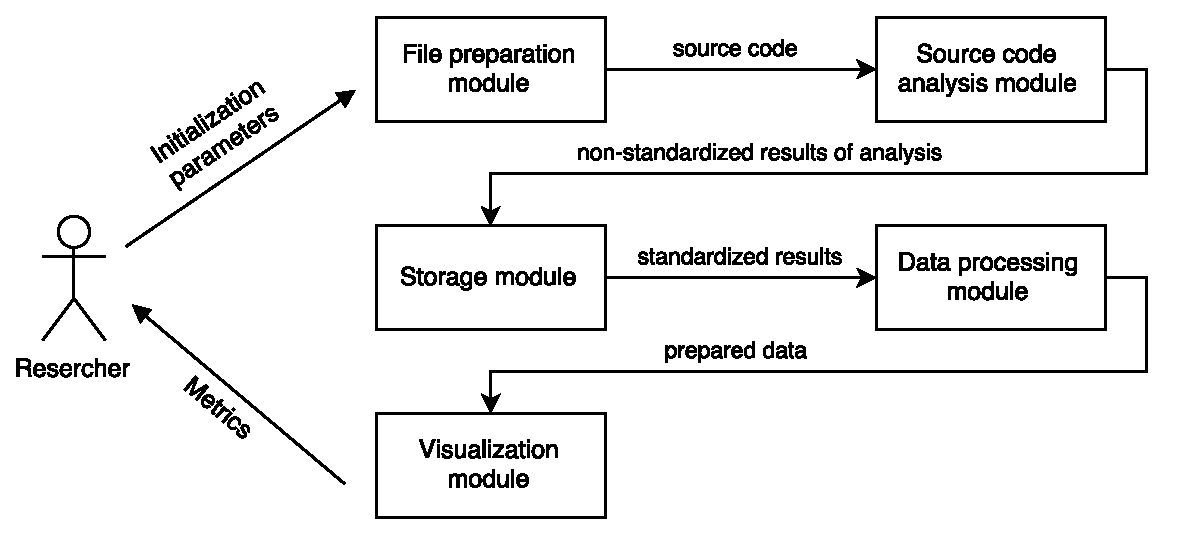
\includegraphics[width=\linewidth]{structscheme}
	\caption{Block diagram of a framework for massive source code analysis using static code analyzers}
	\label{fig:structscheme}
\end{figure}
%

The file preparation module is an entry point for a user. The user defines
all necessary environment for subsequent analysis. This environment consists
of a folder with project source code to be analyzed, a set of analyzers
to utilize, a set of excluded analyzer rules and so on.

After setting up the environment and starting the application system begins
to perform source code analysis. It's worth to mention that we chose Python
as a reference programming language, mainly, because Python has a lot of
scientific libraries for data processing, visualization and so on. We decided
to start off with a preexisting set of source code analyzers and then write
our own custom solution if it becomes needed. Thus, our first task was to
compare existing open source implementations of static source code
analyzing tools for Python language.

There is only a limited number of code analysis frameworks for Python with an ability
to plug different static code analyzers. Namely, they are Coala \cite{item13},
Pylama \cite{item14} and Flake8 \cite{item15}.

We defined the following set of parameters to compare these frameworks:
popularity among Github \cite{item16} users, CPU and RAM utilization, ability to
parallelize process of analysis and time required to process the same set of projects.

Since Flake8 is designed to perform style guide enforcements only and does not
have an ability to disable standard plugins easily we excluded it from further comparison.

Coala provides a uniform CLI interface for code style checking and code
improvement. Coala uses a set of plugins (called "bears") for various
programming languages. It's also possible to extend a standard set of
plugins with a custom plugin.

Pylama is a code auditing tool for Python and JavaScript programming
languages. It is not as feature rich as Coala due to lesser popularity
on Github and lower number of active contributors and code commits.

We used a virtual machine with 3Gb of RAM, 3 CPU cores and Ubuntu 14.04
installed as a test host. We chose a relatively small sample project (consisted
of roughly 130 files) and configured two plugins in both Coala and Pylama.
Processing time took 112 seconds for Coala and 183 seconds for Pylama.

But it turned out that the most important metric was RAM utilization. We created
a graphical representation of OS memory usage on Fig.~\ref{fig:memusage}.

%
\begin{figure}
	\centering
	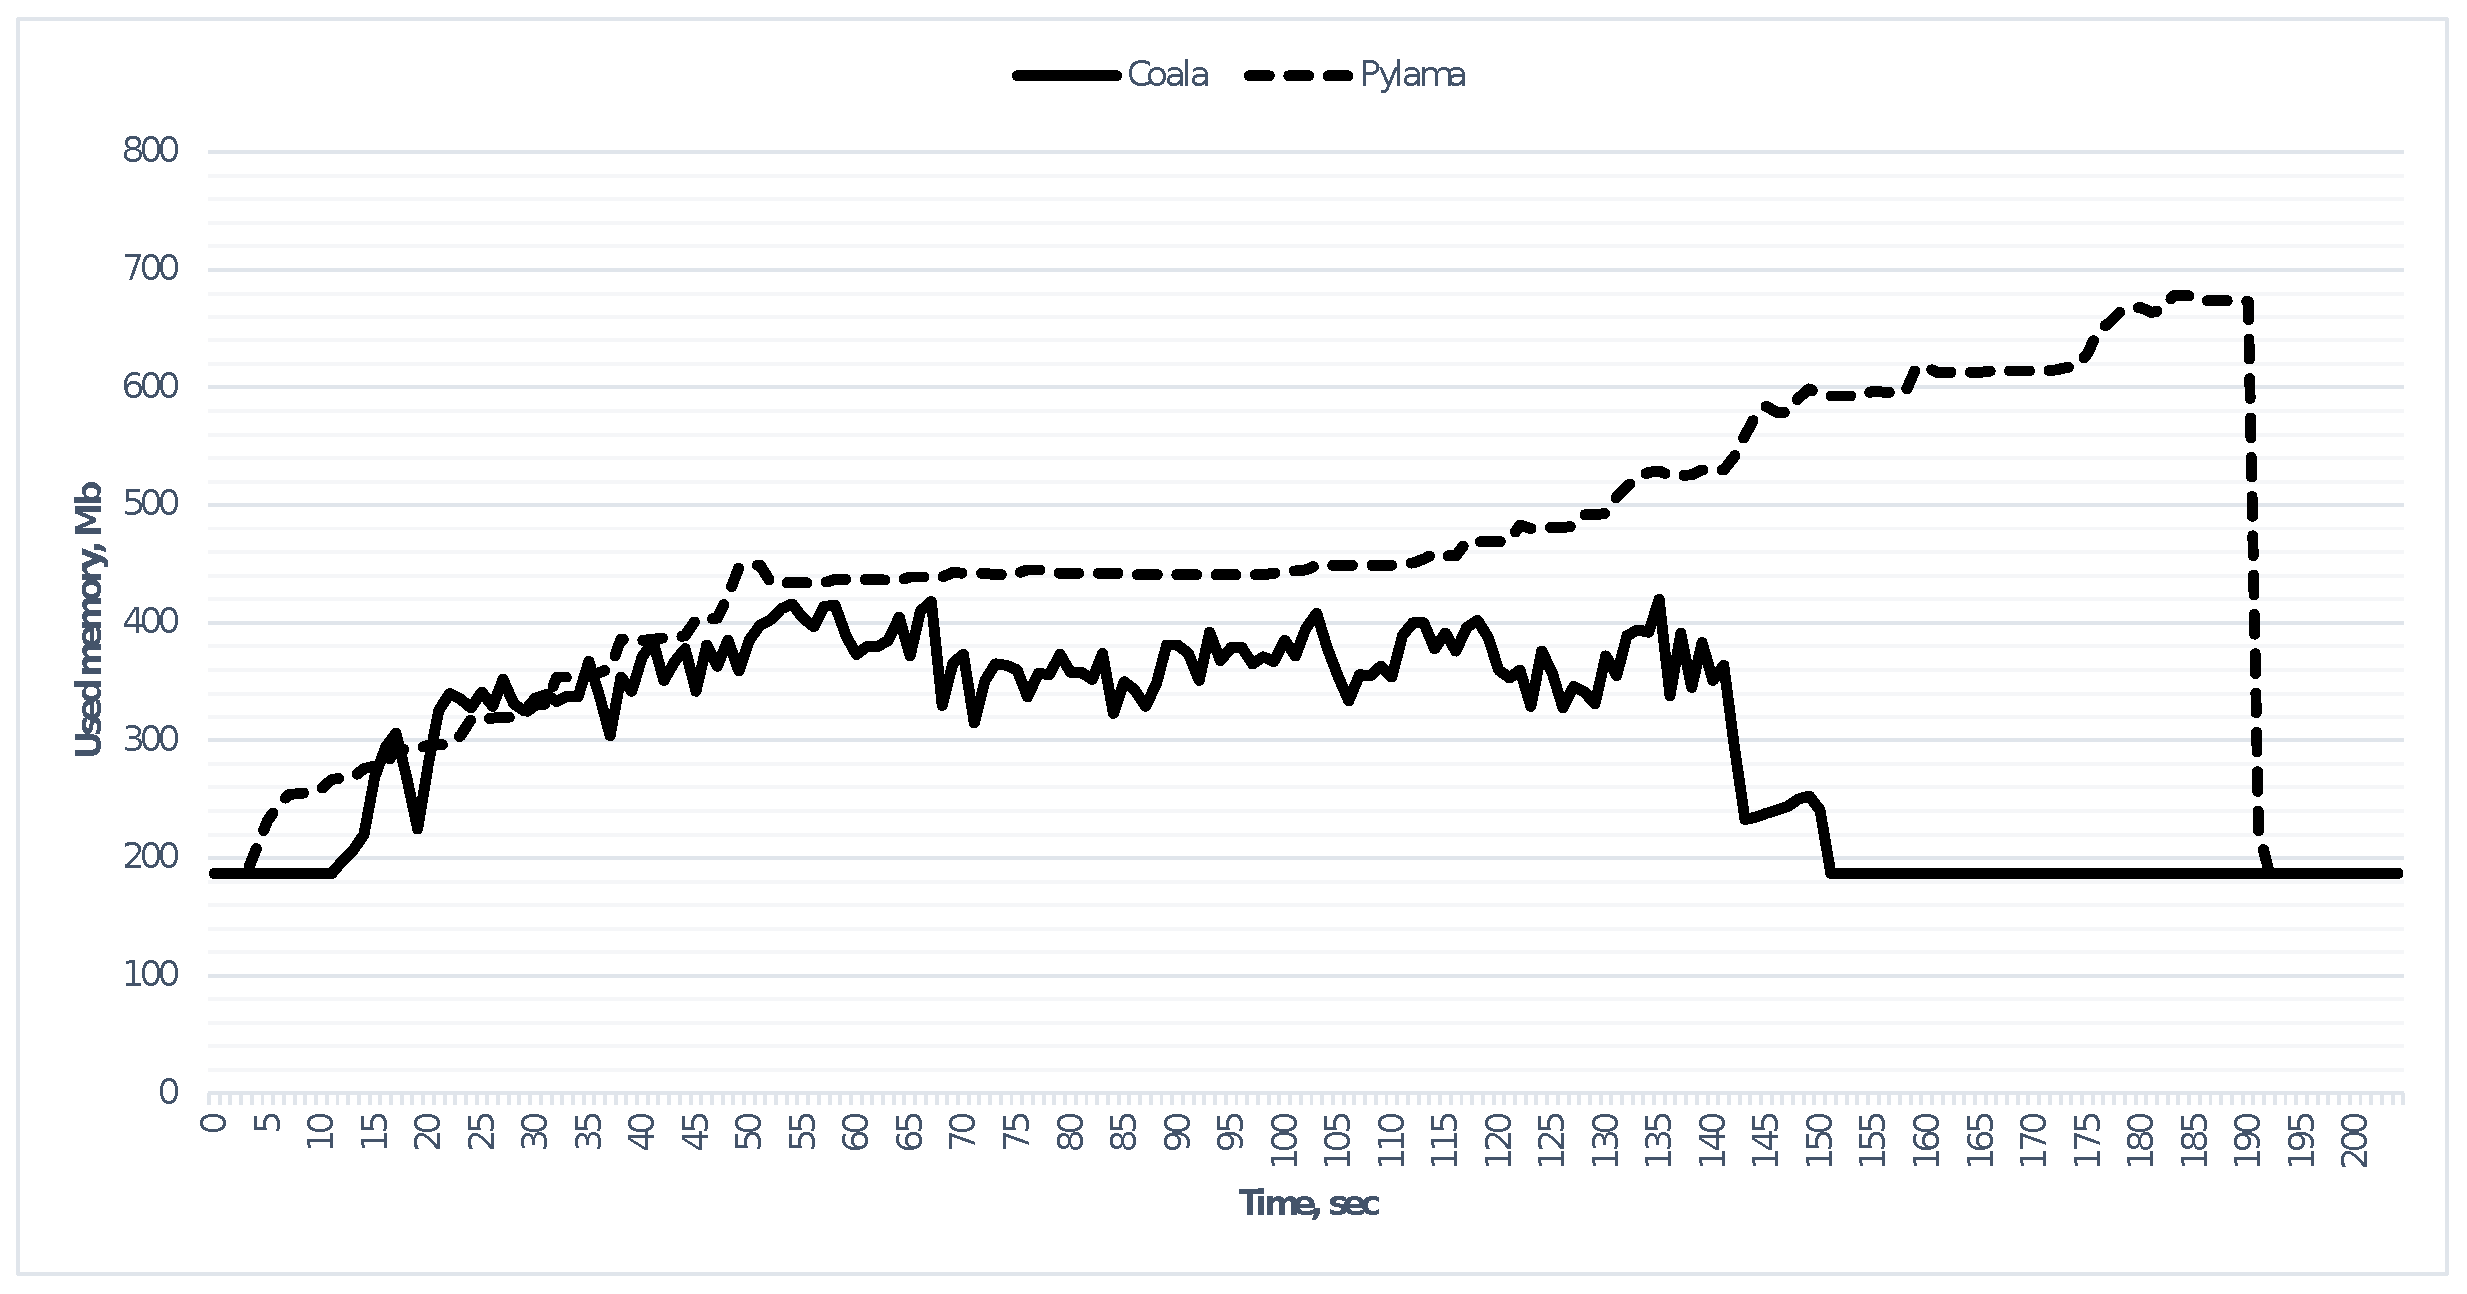
\includegraphics[width=\linewidth]{memusage}
	\caption{OS memory usage when analyzing a single project by Coala and Pylama}
	\label{fig:memusage}
\end{figure}
%

Pylama constantly accumulates information about errors so needed RAM grows
almost linearly. This leads to a critical defect that reveals as total RAM
exhaustion. Operating system forcibly terminates Pylama then. Coala does not
accumulate errors and flushes information on errors to stdout periodically, so
the RAM does not exhaust.

Combined comparison results are presented in Table~\ref{tab:compare}. Based on
this results we decided to use Coala as a base framework for future works.
Another possible option is to patch Pylama.

%
\begin{table}
	\caption{\label{tab:compare}Comparison of Coala and Pylama}
	\begin{center}
		\begin{tabular}{p{5cm}|P{2.5cm}|P{2.5cm}}
			\hline
			~                              & Coala & Pylama \\ \hlineB{2}
			Popularity among github users  & +     & -      \\ \hline
			CPU usage                      & +     & +      \\ \hline
			RAM usage                      & +     & -      \\ \hline
			Parallel processing            & +     & -      \\ \hline
			Analysis time                  & +     & -      \\ \hline
		\end{tabular}
	\end{center}
\end{table}
%

Next planned step is to process results of analysis by a parsing module
and to standartize them. We are going to store standartized analysis results to
a database. We plan to evaluate a number of relational (e.g. PostgreSQL) and
non-relational databases (e.g. HBase and Cassandra).

We designed a data model and represented it as an ER diagram (Fig.~\ref{fig:dbscheme}).

%
\begin{figure}
	\centering
	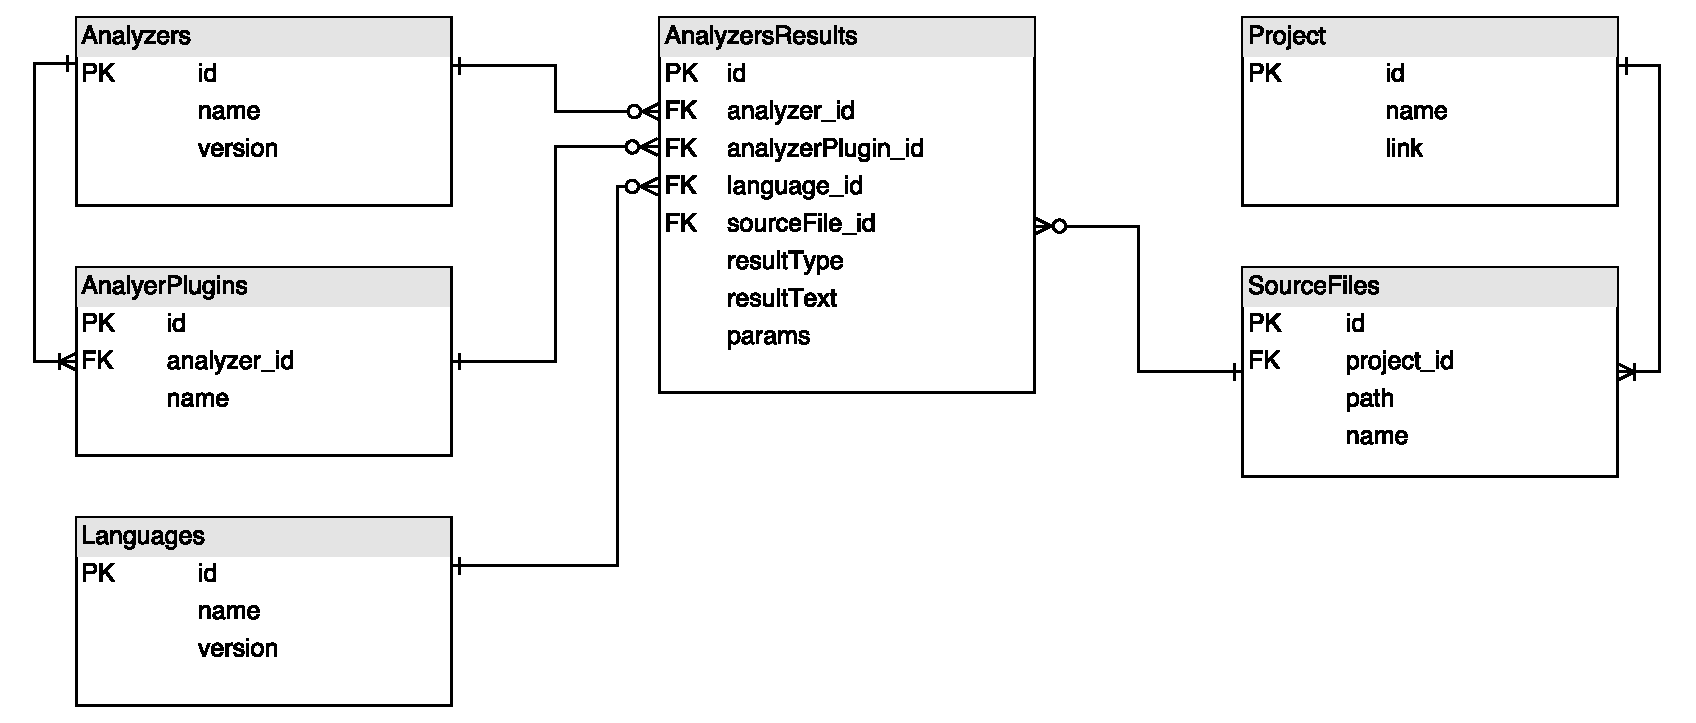
\includegraphics[width=\linewidth]{dbscheme}
	\caption{The database schema for storing source code analysis results}
	\label{fig:dbscheme}
\end{figure}
%

Analysis results are going to be represented as numerical metrics stored in
tables. Next step is to create a separate module to interpret these raw
standartizes results. The last step is to visualize results by a request of
end user initiated code analysis. Thus, different types of comparisons can be
done on visualization step \cite{item17}. For example, comparison can be based
on chronological characteristics of objects or we can perform per component comparison.

Resulting infographics can be presented in various forms, e.g. matrixes, maps,
figures, graphs and diagrams.

\section{Future work}

We defined an overall structure of the system so the next step is
to build a working prototype suitable for massive code analysis. Also
we are going to define a more strict set of metrics and to start
visualizing them. Some of methods of visualizing results of measuring
quality of program products are described in \cite{item18,item19,item20}.

\section{Conclusion}

A problem of controlling, measuring and predicting code quality is actual
at the moment and will become even more actual in the future. Software
developers working on big projects need measurable code quality-related
metrics to improve their process. End users and other third parties need
these metrics to choose a product of best possible quality and for various
other needs. Solving this problem requires a proper instrument which scales
well and produces well-defined and predictable results. Authors of this paper
proposed an approach of creating this instrument, described its architecture
and chose a set of tools as a base to implement it.

\begin{thebibliography}{4}

\bibitem{item01} Zvezdin, S.V.: Problems of measuring program code
  quality. J. South Urals State Univ. 2 (178), (2010)

\bibitem{item02} Irigoyen Ferreiro Ferreira A. et al.: Applying
  ISO 9001:2000, MPS. BR and CMMI to achieve software process
  maturity: BL informatica's pathway. In: Proceedings of the 29th international
  conference on Software Engineering, pp. 642--651. IEEE Computer Society (2007)

\bibitem{item03} Kaigorodtsev, G.I.: Introduction to measurement theory and
  metrology of programs. NGTU Publishing, Novosibirsk (2011)
  
\bibitem{item04} Fernandez, E.B., Larrondo-Petrie, M.M., Sorgente, T.,
  VanHilst, M.: A methodology to develop secure systems using patterns. In:
  Integrating Security and Software Engineering: Advances and Future Vision;
  Mouratidis, H., Giorgini, P. (eds.) IGI Global Group. pp. 107--126. Hershey,
  PA, USA (2006)
 
\bibitem{item16} GitHub: Social coding, \url{https://github.com}

\bibitem{item05} Louridas, Panagiotis. "Static code analysis." IEEE Software 23.4 (2006): 58-61.

\bibitem{item06} Shabtai, Asaf, Yuval Fledel, and Yuval Elovici. "Automated static code analysis for classifying android applications using machine learning." Computational Intelligence and Security (CIS), 2010 International Conference on. IEEE, 2010.

\bibitem{item07} Antunes, Nuno, and Marco Vieira. "Comparing the effectiveness of penetration testing and static code analysis on the detection of sql injection vulnerabilities in web services." Dependable Computing, 2009. PRDC'09. 15th IEEE Pacific Rim International Symposium on. IEEE, 2009.

\bibitem{item08} Baca, Dejan, et al. "Static code analysis to detect software security vulnerabilities-does experience matter?." Availability, Reliability and Security, 2009. ARES'09. International Conference on. IEEE, 2009.

\bibitem{item09} Zitser, Misha, Richard Lippmann, and Tim Leek. "Testing static analysis tools using exploitable buffer overflows from open source code." ACM SIGSOFT Software Engineering Notes. Vol. 29. No. 6. ACM, 2004.

\bibitem{item10} Menzies, Tim, Jeremy Greenwald, and Art Frank. "Data mining static code attributes to learn defect predictors." IEEE transactions on software engineering 33.1 (2007).

\bibitem{item11} Moser, Andreas, Christopher Kruegel, and Engin Kirda. "Limits of static analysis for malware detection." Computer security applications conference, 2007. ACSAC 2007. Twenty-third annual. IEEE, 2007.

\bibitem{item12} Chernonozhkin, S.K.: Metrics of program complexity (A review).
  In: Systems Informatics 5 pp. 188--227. (1997)
  
\bibitem{item13} Coala - Linting and fixing code for all languages, \url{http://coala.io}

\bibitem{item14} Pylama - code audit tool for Python and JavaScript, \url{https://pylama.readthedocs.io}

\bibitem{item15} Flake8 - your tool for style guide enforcement, \url{http://flake8.pycqa.org}

\bibitem{item17} Nefedyeva, K.V.: Infographics and data visualization in
  analytics. In: Proceedings of Saint-Petersburg State University of Culture and
  Arts 197 (2013)

\bibitem{item18} Lanza, Michele, and Radu Marinescu. Object-oriented metrics in practice: using software metrics to characterize, evaluate, and improve the design of object-oriented systems. Springer Science \& Business Media, 2007.

\bibitem{item19} Lanza, Michele, and Stéphane Ducasse. "Polymetric views-a lightweight visual approach to reverse engineering." IEEE Transactions on Software Engineering 29.9 (2003): 782-795.

\bibitem{item20} Lanza, Michele, and Stéphane Ducasse. "Understanding software evolution using a combination of software visualization and software metrics." In Proceedings of LMO 2002 (Langages et Modèles à Objets. 2002.

\end{thebibliography}

\end{document}
